

%%%%%%%%%%%%%%%%%%%%%%%%%%%%% Define Article %%%%%%%%%%%%%%%%%%%%%%%%%%%%%%%%%%
\documentclass[conference]{IEEEtran}
%%%%%%%%%%%%%%%%%%%%%%%%%%%%%%%%%%%%%%%%%%%%%%%%%%%%%%%%%%%%%%%%%%%%%%%%%%%%%%%

%%%%%%%%%%%%%%%%%%%%%%%%%%%%% Using Packages %%%%%%%%%%%%%%%%%%%%%%%%%%%%%%%%%%
\usepackage{geometry}
\usepackage{graphicx}
\usepackage{amssymb}
\usepackage{amsmath}
\usepackage{amsthm}
    
\usepackage{empheq}
\usepackage{mdframed}
\usepackage{booktabs}
\usepackage{lipsum}
\usepackage{graphicx}
\usepackage{color}
\usepackage{psfrag}
\usepackage{pgfplots}
\usepackage{bm}
\usepackage[spanish]{babel}
\usepackage[utf8]{inputenc} % Codificación UTF-8
\usepackage{amsmath}        % Soporte para ecuaciones matemáticas
\usepackage{graphicx}       % Manejo de imágenes
\usepackage{hyperref}       % Hipervínculos
\usepackage{caption}        % Formato para figuras
\usepackage{multirow}
\usepackage{subcaption}
\usepackage{biblatex}
\usepackage{csquotes}
\usepackage{bookmark}
%%%%%%%%%%%%%%%%%%%%%%%%%%%%%%%%%%%%%%%%%%%%%%%%%%%%%%%%%%%%%%%%%%%%%%%%%%%%%%%

% Other Settings

%%%%%%%%%%%%%%%%%%%%%%%%%% Page Setting %%%%%%%%%%%%%%%%%%%%%%%%%%%%%%%%%%%%%%%
\geometry{a4paper, margin=1in}

%%%%%%%%%%%%%%%%%%%%%%%%%% Define some useful colors %%%%%%%%%%%%%%%%%%%%%%%%%%
\definecolor{ocre}{RGB}{243,102,25}
\definecolor{mygray}{RGB}{243,243,244}
\definecolor{deepGreen}{RGB}{26,111,0}
\definecolor{shallowGreen}{RGB}{235,255,255}
\definecolor{deepBlue}{RGB}{61,124,222}
\definecolor{shallowBlue}{RGB}{235,249,255}
%%%%%%%%%%%%%%%%%%%%%%%%%%%%%%%%%%%%%%%%%%%%%%%%%%%%%%%%%%%%%%%%%%%%%%%%%%%%%%%

%%%%%%%%%%%%%%%%%%%%%%%%%% Define an orangebox command %%%%%%%%%%%%%%%%%%%%%%%%
\newcommand\orangebox[1]{\fcolorbox{ocre}{mygray}{\hspace{1em}#1\hspace{1em}}}
%%%%%%%%%%%%%%%%%%%%%%%%%%%%%%%%%%%%%%%%%%%%%%%%%%%%%%%%%%%%%%%%%%%%%%%%%%%%%%%

%%%%%%%%%%%%%%%%%%%%%%%%%%%% English Environments %%%%%%%%%%%%%%%%%%%%%%%%%%%%%
\newtheoremstyle{mytheoremstyle}{3pt}{3pt}{\normalfont}{0cm}{\rmfamily\bfseries}{}{1em}{{\color{black}\thmname{#1}~\thmnumber{#2}}\thmnote{\,--\,#3}}
\newtheoremstyle{myproblemstyle}{3pt}{3pt}{\normalfont}{0cm}{\rmfamily\bfseries}{}{1em}{{\color{black}\thmname{#1}~\thmnumber{#2}}\thmnote{\,--\,#3}}
\theoremstyle{mytheoremstyle}
\newmdtheoremenv[linewidth=1pt,backgroundcolor=shallowGreen,linecolor=deepGreen,leftmargin=0pt,innerleftmargin=20pt,innerrightmargin=20pt,]{theorem}{Theorem}[section]
\theoremstyle{mytheoremstyle}
\newmdtheoremenv[linewidth=1pt,backgroundcolor=shallowBlue,linecolor=deepBlue,leftmargin=0pt,innerleftmargin=20pt,innerrightmargin=20pt,]{definition}{Definition}[section]
\theoremstyle{myproblemstyle}
\newmdtheoremenv[linecolor=black,leftmargin=0pt,innerleftmargin=10pt,innerrightmargin=10pt,]{problem}{Problem}[section]
%%%%%%%%%%%%%%%%%%%%%%%%%%%%%%%%%%%%%%%%%%%%%%%%%%%%%%%%%%%%%%%%%%%%%%%%%%%%%%%

%%%%%%%%%%%%%%%%%%%%%%%%%%%%%%% Plotting Settings %%%%%%%%%%%%%%%%%%%%%%%%%%%%%
\usepgfplotslibrary{colorbrewer}
\pgfplotsset{width=8cm,compat=1.9}
%%%%%%%%%%%%%%%%%%%%%%%%%%%%%%%%%%%%%%%%%%%%%%%%%%%%%%%%%%%%%%%%%%%%%%%%%%%%%%%

%%%%%%%%%%%%%%%%%%%%%%%%%%%%%%% Title & Author %%%%%%%%%%%%%%%%%%%%%%%%%%%%%%%%
\author{\IEEEauthorblockN{Daniel Fernando Aranda Contreras}
\IEEEauthorblockA{Escuela E3T, Universidad Industrial de Santander\\
Correo electrónico: \{daniel2221648\}@correo.uis.edu.co}}

%%%%%%%%%%%%%%%%%%%%%%%%%%%%%%%%%%%%%%%%%%%%%%%%%%%%%%%%%%%%%%%%%%%%%%%%%%%%%%%
    \begin{document}
        % Título
        \title{\uppercase{Análisis y Especificaciones de diagrama electrico en un sistema Residencial}}
        \maketitle
        % Resumen
        % Palabras clave        
        \begin{IEEEkeywords}
            Transformador, Tensión, Corriente alterna, Distribución de energía eléctrica, Especificaciones técnicas, Medidor, Consumo de energía, Kilovatios-hora (kWh), Caja de relés, Interruptores automáticos, Flujos de electricidad, Seguridad eléctrica, Diagrama de conexión, Instalación eléctrica, Electrodomésticos, Prevención de incendios, Sistema eléctrico residencial, Mantenimiento de dispositivos eléctricos.
        \end{IEEEkeywords}




        \section{Transformador}
        
        \subsection{Definición y Función}
        Un transformador es un dispositivo electromagnético que permite transferir energía eléctrica entre dos o más circuitos a través de la inducción magnética. Se utiliza principalmente para aumentar (transformador elevador) o disminuir (transformador reductor) el voltaje de la corriente alterna (CA), facilitando así la transmisión y distribución de electricidad. En la figura \ref{fig:Tansformador} se muestra un transformador reductor.
        \begin{figure}[h] % 'h' indica que la imagen se coloca aquí
            \centering
            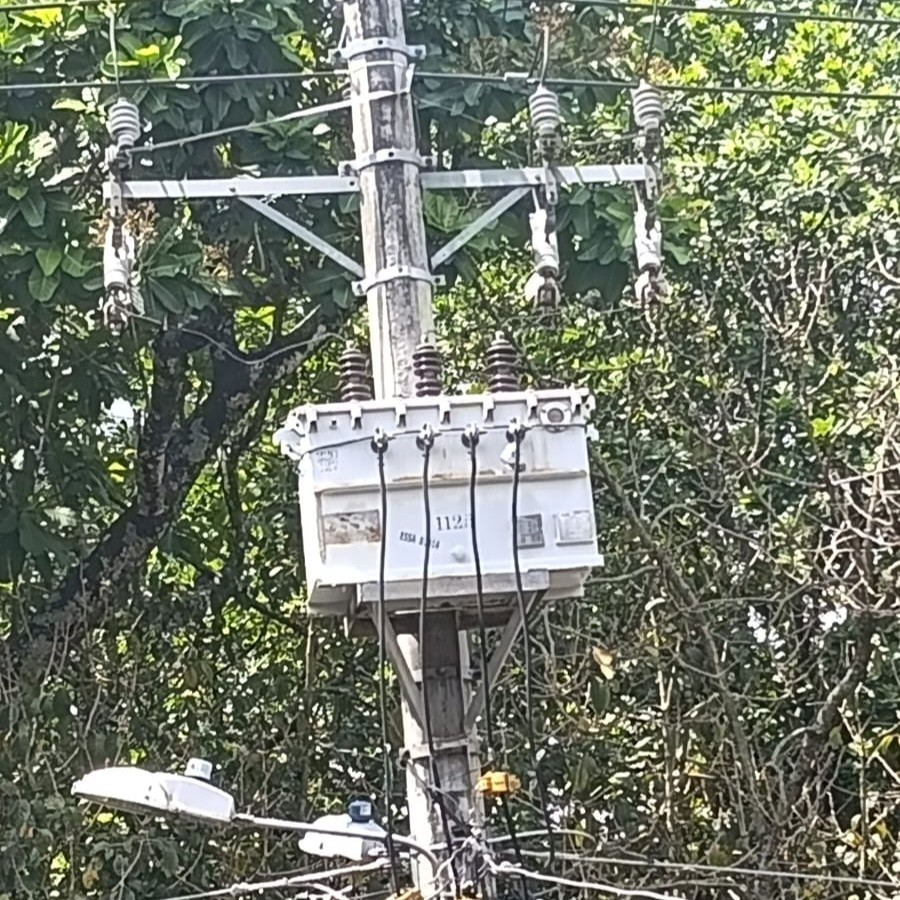
\includegraphics[width=0.5\textwidth]{img/Transformador.jpg} % Cambia la ruta a tu imagen
            \caption{Transformador Reductor de mi hogar.}
            \label{fig:Tansformador}
        \end{figure}


        \subsection{Especificaciones Técnicas}
        \begin{itemize}
            \item \textbf{Tipo de Transformador:} trifásico.
            \item \textbf{Potencia Nominal:} 112.5 (kVA).
            \item \textbf{Relación de Transformación:} Del lado primario baja/media tensión y secundario 110-120 V.
            \item \textbf{Aislamiento:} Puede que sea papel cubierto en resina epoxica.
        \end{itemize}
        
        \subsection{Importancia}
        El transformador en este caso de baja, ajusta la tensión eléctrica, garantizando su seguridad y adecuación para el uso en hogares.
        
        \section{Medidor}
        
        \subsection{Definición y Función}
        El medidor de electricidad mide el consumo de energía eléctrica en una propiedad. Registra la cantidad de kilovatios-hora (kWh) utilizados. Para este caso no tuve acceso al medidor de mi hogar, pero se muestra un ejemplo en la figura \ref{fig:medidor}.
        
        \begin{figure}[h] % 'h' indica que la imagen se coloca aquí
            \centering
            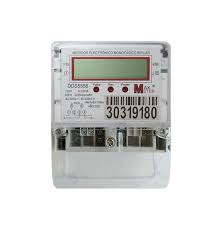
\includegraphics[width=0.5\textwidth]{img/Medidor digital.jpg} % Cambia la ruta a tu imagen
            \caption{Medidor digital.}
            \label{fig:medidor}
        \end{figure}



        \subsection{Especificaciones Técnicas}
        \begin{itemize}
            \item \textbf{Tipo de Medidor:} digital.
            \item \textbf{Rango de Medición:} desconocido.
            \item \textbf{Conectividad:} Permite transmisión de datos para lectura remota.
        \end{itemize}
        
        \subsection{Importancia}
        El medidor permite a las compañías eléctricas facturar el consumo y ayuda a los usuarios a gestionar su uso de energía.
        
        \section{Caja de Relés}
        
        \subsection{Definición y Función}
        La caja de relés alberga interruptores automáticos o relés que controlan el flujo de electricidad, protegiendo contra sobrecargas.
        En la figura \ref{fig:tablero} se muestra un ejemplo de un tablero de distribución residencial.
        \begin{figure}[h] % 'h' indica que la imagen se coloca aquí
            \centering
            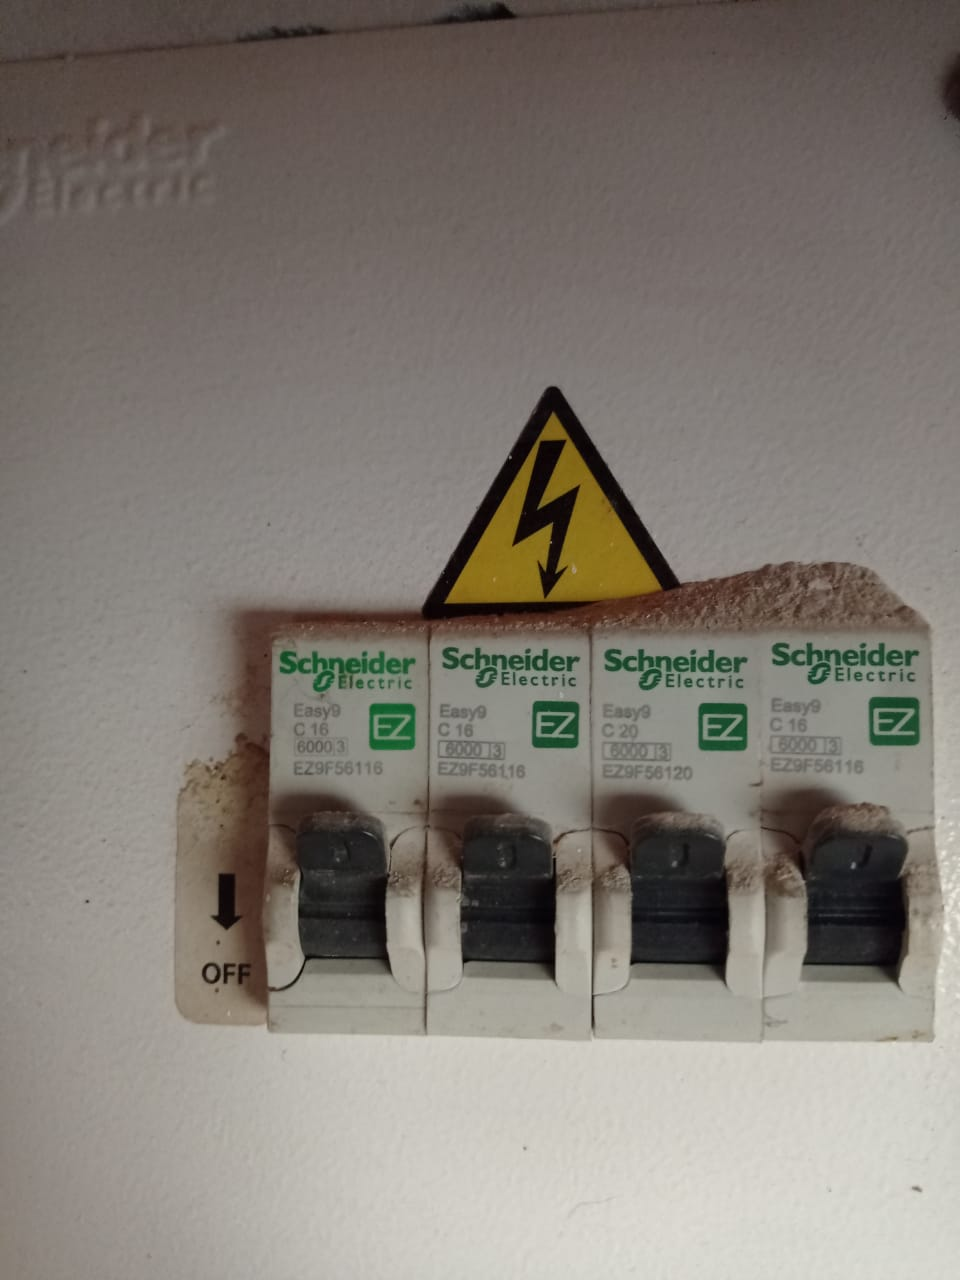
\includegraphics[width=0.5\textwidth]{img/tablero de distribucion.jpg} % Cambia la ruta a tu imagen
            \caption{Tablero de Distrubución Residencial.}
            \label{fig:tablero}
        \end{figure}

        \subsection{Especificaciones Técnicas}
        \begin{itemize}
            \item \textbf{Tipo de Relés/Interruptores:} Interruptor termomagnético.
            \item \textbf{Capacidad de Corriente:} 16A 10kA curva C
            \item \textbf{Número de Circuitos:} Varía según diseño de la instalación.
        \end{itemize}
        
        \subsection{Importancia}
        La caja de relés es esencial para la seguridad del sistema eléctrico del hogar, previniendo daños en electrodomésticos y reduciendo riesgos de incendios.
                
        \subsection{Diagrama de Conexión}
        Obtenido de link: \url{https://likinormas.enelcol.com.co/normas/centros-de-transformacion
        -para-redes-aereas-urbanos-y-rurales/centros-de-transformacion-aereos-urbanos-trifasicos/
        ctu516-1-diagrama-unifilar-instalacion-de-transformador-de-distribucion-bifilar-11-400-120
        -240-v}
        \begin{figure}[h] % 'h' indica que la imagen se coloca aquí
            \centering
            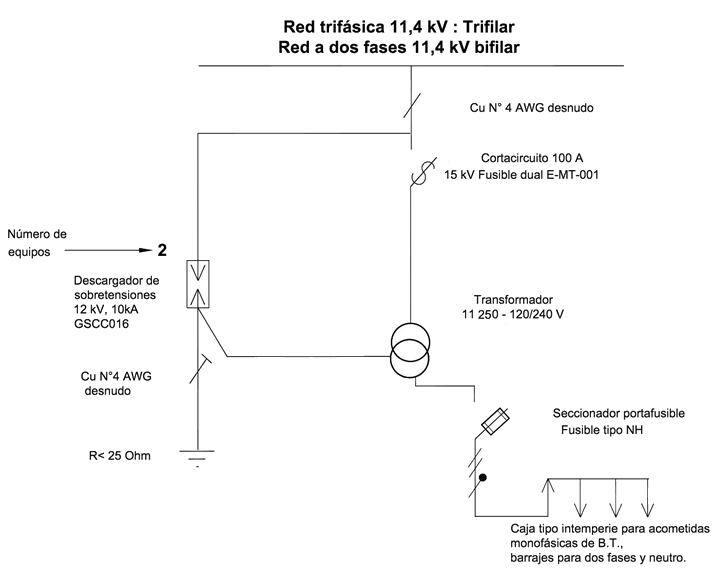
\includegraphics[width=0.5\textwidth]{img/Diagrama.png} % Cambia la ruta a tu imagen
            \caption{Diagrama de conexión del circuito Residencial.}
            \label{fig:Residencial}
        \end{figure}

        \section{Conclusión}
        Finalmente, el sistema eléctrico residencial es un conjunto de dispositivos que permiten la distribución de energía eléctrica de manera segura y eficiente. La correcta selección y mantenimiento de estos dispositivos es fundamental para garantizar la seguridad y el buen funcionamiento del sistema.

    \end{document}  
